\subsubsection{Les cases}
La carte du monde est constituée de cinq types de cases hexagonales : les salles infos, les salles de TD, les amphitheâtres, le self et les extérieures.
Il y a de un à trois self selon le type de map choisi, la moitié des cases sont des extérieurs, et le reste est réparti équitablement entre les autres types de cases.
\begin{figure}[!h]
\centering
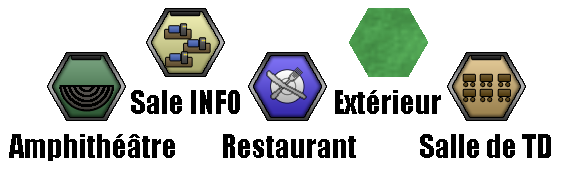
\includegraphics[width=.7\textwidth]{Parties/Images/Terrains.png}
\caption{Les différentes cases, comme elles sont représentées dans le jeu}
\label{fig:Terrains}
\end{figure}

\subsubsection{Les différents types de jeu}
Il existe trois cartes différentes :
\begin{itemize}
\item Démo : 2 joueurs, 6*6 cases, 5 tours, 4 unités par joueur.
\item Petite : 2 joueurs, 10*10 cases, 20 tours, 6 unités par joueur.
\item Démo : 2 joueurs, 14*14 cases, 30 tours, 8 unités par joueur.
\end{itemize}